
%(BEGIN_QUESTION)
% Copyright 2011, Tony R. Kuphaldt, released under the Creative Commons Attribution License (v 1.0)
% This means you may do almost anything with this work of mine, so long as you give me proper credit

This amount of vacuum (negative pressure) in this knock-out drum is controlled by varying the compressor's bypass valve:

$$\includegraphics[width=15.5cm]{i02489x01.eps}$$

An operator tells you there is a problem with this system, though: the vacuum gauge near the pressure transmitter registers -6.9 PSI, even though the controller faceplate registers -8.0 PSI which is the same as the setpoint.  The same operator notes that the control valve position is approximately 30\% open, with the controller's output bargraph registering 31.4\% open.

\vskip 10pt

Another instrument technician happens to be with you, and recommends the operator place the pressure controller in manual mode to ``stroke-test'' the control valve.  Explain why this test would be a waste of time, and propose a better test for helping to pinpoint the location of the fault.

\vskip 20pt \vbox{\hrule \hbox{\strut \vrule{} {\bf Suggestions for Socratic discussion} \vrule} \hrule}

\begin{itemize}
\item{} A valuable principle to apply in a diagnostic scenario such as this is {\it correspondence}: identifying which field variables correspond with their respective controller faceplate displays, and which do not.  Apply this comparative test to the scenario described, and use it to explain why the technician's proposed test was probably not the best first step.
\item{} A problem-solving technique useful for analyzing control systems is to mark the PV and SP inputs of all controllers with ``+'' and ``$-$'' symbols, rather than merely label each controller as ``direct'' or ``reverse'' action.  Apply this technique to the control strategy shown here, identifying which controller input(s) should be labeled ``+'' and which controller input(s) should be labeled ``$-$''.
\item{} Predict the effects resulting from one of the transmitters in this system failing with either a {\it high} or a {\it low} signal.
\item{} For those who have studied level measurement, explain how the level transmitter (which is nothing more than a DP transmitter) senses liquid level inside the knock-out drum.
\end{itemize}

\underbar{file i02489}
%(END_QUESTION)





%(BEGIN_ANSWER)

The reason that the technician's proposed test would have been a waste of time is because the issue at hand is a significant disagreement between the vacuum gauge and the controller display.  No valve problem or controller output problem could cause this to happen.
 
A far better test would be to place the pressure controller in manual mode, then vent the pressure transmitter to check that the controller reads 0 PSI.  If there is a transmitter calibration problem, it will likely appear as a zero error (not reading 0 PSI at 0 PSI).  

Alternatively, one could also perform the same test on the vacuum gauge to see if it is in error.

\vskip 10pt

The level controller needs to be direct-acting.  The pressure controller needs to be reverse-acting.

\vskip 10pt

Although there is a discrepancy between the controller's output (displayed) and the actual valve position, an error of (approximately) 1.4\% is nothing to worry about.  In fact, so long as the valve is somewhere within its throttling range, the controller should be able to hold the PV equal to SP.


%(END_ANSWER)





%(BEGIN_NOTES)


%INDEX% Basics, control loop troubleshooting: isolating area of fault by correspondence

%(END_NOTES)


